\documentclass[dvipdfmx,11pt]{beamer}
%\graphicspath{{fig_tab/os_presentation/20201215/}}
\usepackage{lipsum}
\usetheme{Verona}
\usepackage{bxdpx-beamer}
\usepackage{pxjahyper}
\usepackage{minijs}
\usepackage{mathpazo}
\usepackage{amsmath,amssymb}
\usepackage{graphicx}
\usepackage{array}
\usepackage{tikz}
\usepackage{wrapfig}
\usepackage{float}
\usepackage{here}
\usepackage{lscape}
\usepackage{ascmac}
\usepackage{tabularx}
\renewcommand{\kanjifamilydefault}{\gtdefault}
\hypersetup{% hyperrefオプションリスト
 setpagesize=false,
 bookmarksnumbered=true,%
 bookmarksopen=true,%
 colorlinks=true,%
 linkcolor=blue,
 citecolor=blue,
 urlcolor = magenta
}
\setbeamertemplate{navigation symbols}{}

\title[Calderon, Fouka, and Tabellini, 2022]{Racial Diversity and Racial Policy Preferences: \\
The Great Migration and Civil Rights}
\subtitle{Calderon, Fouka, and Tabellini (2022)}
\author{Reviewed by R. TANJI}
\date[6/12/2022 OS Semi.]{July 12th, 2022 \\ Ohtake-Sasaki Seminar}
\institute[]{Osaka University, Graduate School of Economics}

\begin{document}

\begin{frame}\frametitle{}
\titlepage
\end{frame}

\begin{frame}{Abstract}
  \begin{itemize}
    \item Research Question: Is the Great Migration is causally linked with support for civil rights?
    \begin{itemize}
      \item Between 1940 and 1970, more than 4 million African Americans moved from the South to the North of the US.
      \item At the same period witnessed the struggle and eventual success of the civil rights movements: the
      National Association for the Advancement of Colored People (NAACP) and the Congress of
      Racial Equality (CORE).
    \end{itemize}
    \item The (Second) Great Migration: Shift-share IV of Black inflows
    \begin{itemize}
      \item raised support for the Democratic Party
      \item increased Congress members' propensity to promote civil rights legislation
      \item encouraged pro-civil rights activism outside the US South
    \end{itemize} 
  \end{itemize}
\end{frame}

\frame{\tableofcontents}

\section{Introduction}
\frame{\sectionpage}

\begin{frame}{Literature}
  \begin{itemize}
    \item The effect of the inflow of Black voters is puzzling.
    \begin{itemize}
      \item may have shifted northern politicians incentives to introduce civil rights legislation.
      \begin{itemize}
        \item African Americans were largely disenfranchised in the South but faced no voting restrictions in the North
        \item Black population might have also expanded the organizational capacity of the Black civil rights movement (McAdam, 1982)
      \end{itemize}
      \item may have generated political opposition among northern whites
      \begin{itemize}
        \item racial diversity often triggers backlash among members of the majority group (Alesina, Baqir and Easterly, 1999; Enos, 2016; Dustmann, Vasiljeva and Damm, 2019).
      \end{itemize}
    \end{itemize}
    \item in Economic Literature: 
    \begin{itemize}
      \item the Great Migration increased residential segregation (Boustan, 2010)
      \item lowered the economic and social mobility of African Americans in the long run (Derenoncourt, 2022).
    \end{itemize}
  \end{itemize}
\end{frame}

\begin{frame}{}
  \begin{figure}
    \centering
    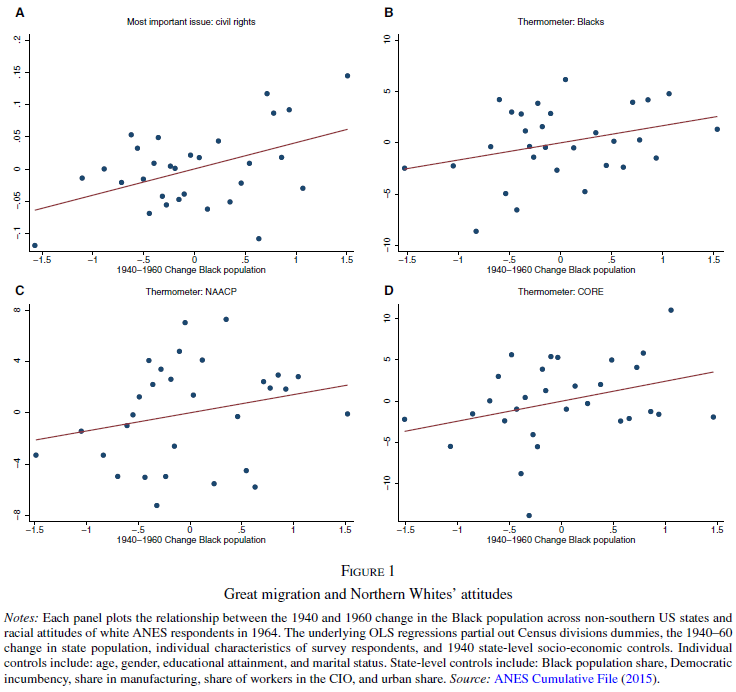
\includegraphics[scale = .45]{fig_tab/os20220708/F1.png}
  \end{figure}
\end{frame}

\begin{frame}{Research Design}
  \begin{itemize}
    \item This article shows a causal relationship between the Black inflow to northern counties (the Great Migration between 1940-1970) and support for civil rights.
    \begin{itemize}
      \item Potentially endogenous migration: Blacks may have migrated to the counties that shows more support for civil rights.
      \item Shift-share instrument (Card, 2001; Boustan, 2010): the expected number of the Black inflow conditional on the preexisting settlements before 1940.
    \end{itemize}
    \item Using a unique dataset that contains vote share, local support for civil rights, and whites' attitudes in 1,263 non-southern counties (285 Congressional Districts.)
  \end{itemize}
\end{frame}

\begin{frame}{Summary of Results}
  \begin{itemize}
    \item Black in-migration had a strong, positive impact on the Democratic vote share in Congressional elections.
    \begin{itemize}
      \item 1 ppt increase in the Black population share raised the Democratic vote share by 1.8 percentage points (4\% relative to the 1940 mean).
      \item did not lead to white out-migration or to changes in the composition of white residents at the county level.
    \end{itemize}
    \item Congressional Districts that received more African Americans were represented by legislators with a more liberal ideology on racial issues.
    \item These findings are characteristic of the temporal context of their study, but the developments that period (1940-1970) have persisted until today.
  \end{itemize}
\end{frame}

\begin{frame}{Mechanisms}
  \begin{itemize}
    \item The direct effect of Black voters alone is not enough to explain the increase in the Democratic vote share caused by the Great Migration.
    \begin{enumerate}
      \item the changed composition of the electorate (Schickler, 2016; Grant, 2020).
      \item local activism (McAdam, 1982; Biondi, 2021)
    \end{enumerate}
    \item Their dataset shows that approximately 7 white voters would have to switch to the Democratic Party for every 10 Black migrants.
    \begin{itemize}
      \item Historical survey data show that the white in districts that received more Black inflows held more favourable views on race relations.
      \item Not only Black, but also white individuals joined pro-civil rights protests
    \end{itemize}
  \end{itemize}
\end{frame}

\begin{frame}{}
  \begin{enumerate}
    \item Whites had awared of conditions faced by Black people in the South.
    \begin{itemize}
      \item "To get publicity is of the highest strategic
      importance to [Black people]" (Myrdal, 1944).
      \item between 1940 and 1964, northern local newspapers were more likely to report the lynching in counties in the US south if they had received more African Americans.
    \end{itemize}
    \item A cross-race alliance between Black voters and progressive segments of the Democratic coalition (Adams, 1966; Schickler, 2016; Frymer and Grumbach, 2020).
    \begin{itemize}
      \item CORE (Congress of
      Racial Equality) demonstrations were more frequent where, at baseline: the share of whites employed in manufacturing was higher.
      \item the presence of the Congress of Industrial Organizations (CIO) was stronger.
      \item Elections were more competitive.
      \item Pro-civil rights protests were concentrated in counties with a history of lower racial discrimination: presence of miscegenation laws
    \end{itemize}
  \end{enumerate}
\end{frame}

\begin{frame}{Contribution}
  \begin{itemize}
    \item literature in economics and political science: the specific role of the Great Migration.
    \begin{itemize}
      \item the civil rights movement
      \begin{itemize}
        \item consequences of the Civil Rights and the Voting Rights (Cascio, Gordon, Lewis and Reber, 2010; Reber, 2011; Cascio and Washington, 2014; Bernini, Facchini and Testa, 2018; Aneja and Avenancio-Leon, 2019)
        \item the causes of the southern “dealignment” (Besley, Persson and Sturm, 2010; Kousser, 2010; Trende, 2012; Wright, 2013; Kuziemko and Washington, 2018).
        \item Schickler (2016) and Grant (2020): the incorporation of African Americans into the Democratic coalition after the New Deal and the rising pivotal role of Black voters due to the Great Migration.
      \end{itemize}
    \end{itemize}
  \end{itemize}
\end{frame}

\begin{frame}{}
  \begin{itemize}
    \item literature on the relationship between voters' demand and politicians' behaviour
    \begin{itemize}
      \item Lott and Kenny, 1999; Miller, 2008; Mian, Sufi and Trebbi, 2010; Kroth, Larcinese and Wehner, 2016; Caughey and Warshaw, 2018; Jones and Walsh, 2018; Closest to our article, Cascio and Washington (2014): the Voting Rights Act (VRA) shifted the distribution of local spending across southern counties towards Black Americans' preferences
      \item This article expanded on their findings by focusing on the US North rather than the South.
    \end{itemize}
    \item the Great Migration: 
    \begin{itemize}
      \item Previous studies on whites' residential
      decisions, intergenerational mobility, immigrant assimilation, and public finance (Boustan, 2010; Tabellini, 2018; Shertzer and Walsh, 2019; Fouka, Mazumder and Tabellini, 2021; Derenoncourt, 2022)
      \item This article adds its political effects.
    \end{itemize}
  \end{itemize}
\end{frame}

\section{Historical Background}
\frame{\sectionpage}

\begin{frame}{The Great Migration}
  \begin{itemize}
    \item The Second Great Migration: between 1940 and 1970, more than 4 million African Americans left the US South for northern and western destinations.
    \begin{itemize}
      \item The First: From 1915 to 1930, the First Great Migration brought to the North 1.5 million Black migrants.
      \item Most Black migrants moved to urban centres in the Northeast and mid-West, but they also affected the West and less urbanized areas.
    \end{itemize}
    \item Two factors which pulled Black Migrants (Boustan, 2016).
    \begin{enumerate}
      \item economic opportunities
      \begin{itemize}
        \item the outbreak of WWII increased demand for labour in northern and western factories
        \item the mechanization of agricultural harvest
        in the 1940s and 1950s reduced demand for labour in the already depressed southern agricultural sector
      \end{itemize}
      \item racial oppression by the South
      \begin{itemize}
        \item political disenfranchisement
        \item poor working conditions
      \end{itemize}
    \end{enumerate}
  \end{itemize}
\end{frame}

\begin{frame}{}
  \begin{itemize}
    \item Out-migration from the South was strongest during the 1940s, with a Black emigration rate of almost 15\%.
    \item As a result, the US South lost 40\% of its 1940 Black population: the racial profile of the US changed dramatically.
    \begin{itemize}
      \item Black population share of the population in northern and western cities moved from less than 4\% to more than 15\% in just three decades.
    \end{itemize}
    \item Gibson and Jung, 2005: Chicago, Detroit, or St. Louis, where the Black population share of the population moved from 8, 9, and 11\% to 32, 43, and 41\%, respectively 
  \end{itemize}
\end{frame}

\begin{frame}{}
  \begin{figure}
    \centering
    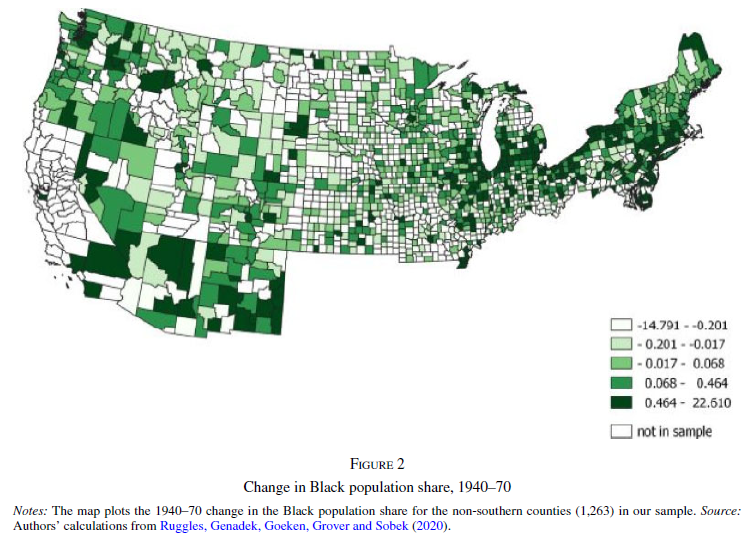
\includegraphics[scale = .5]{fig_tab/os20220708/F2.png}
  \end{figure}
\end{frame}

\begin{frame}{Black Migrants and Northern Politics}
  \begin{itemize}
    \item The demographic change induced by the Great Migration had the potential to alter the political equilibrium
    \item The literature on social movements suggests that the enfranchisement of Black migrants may have increased:
    \begin{itemize}
      \item the organizational capacity of the civil rights movement
      \item the pressure exerted by the Black community on local politicians
    \end{itemize}
    \item Consistently, the number of northern and western counties that had at least one local NAACP (the
    National Association for the Advancement of Colored People (NAACP)).
  \end{itemize}
\end{frame}

\begin{frame}
  \begin{itemize}
    \item Politics:
    \begin{itemize}
      \item The New Deal had better equipped the
      Democratic Party to address the demands of Black Americans outside the US South (Schickler, 2016; Caughey et al., 2020): Democrats in the North
      were more likely to support civil rights bills
      \begin{itemize}
        \item On the other hand, roll call votes do not serve enough information of legislator's preferences.
      \end{itemize}
      \item Signatures on discharge petitions: to circumvent Congressional committees, andmove bills to the floor for a vote.
      \item Non-southern Democratic Congress members were at least 30 percentage points more likely than their Republican counterparts to sign a discharge petition to promote civil rights legislation.
      \item Black residents were also more closely aligned to Democratic's economic agenda than to that of Republicans. 
    \end{itemize}
  \end{itemize}
\end{frame}

\begin{frame}{}
  \begin{figure}
    \centering
    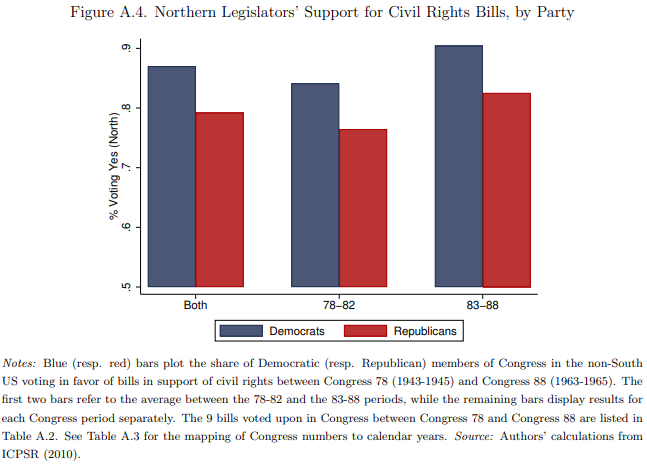
\includegraphics[scale = .5]{fig_tab/os20220708/FA4.png}
  \end{figure}
\end{frame}

\begin{frame}{}
  \begin{figure}
    \centering
    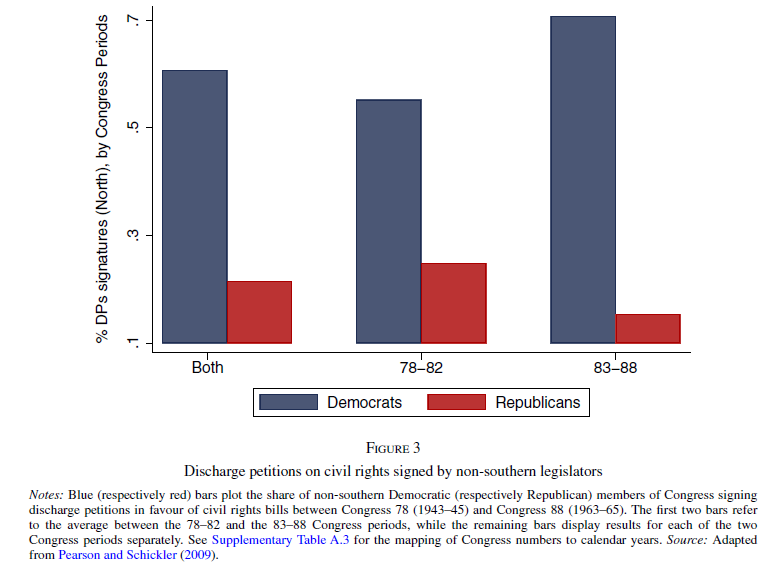
\includegraphics[scale = .5]{fig_tab/os20220708/F3.png}
  \end{figure}
\end{frame}

\section{Data}
\frame{\sectionpage}

\begin{frame}{Dataset}
  \begin{itemize}
    \item Unique dataset composed of 1,263 non-southern counties that include:
    \begin{itemize}
      \item Political outcomes
      \begin{itemize}
        \item the county-level Democratic vote share in Congressional elections from 1940 to 1970
        \item legislators' ideology on racial issues: Gregory and Estrada (2019)'s score
      \end{itemize}
      \item Local support for civil rights
      \begin{itemize}
        \item the presence of chapters of the National Association for the Advancement of Colored People (NAACP): 1940s-1960s from Gregory and Estrada (2019)
        \item number of non-violent demonstrations organized between 1942 and 1970 by the Congress of Racial Equality (CORE)
      \end{itemize}
      \item Whites' attitudes from American National Election Studies (ANES)
      \begin{itemize}
        \item nationally representative survey that elicits individuals' preferences, political ideology, and socioeconomic and demographic characteristics over time. (late 1950s-, state-level)
      \end{itemize}
    \end{itemize}
  \end{itemize}
\end{frame}

\begin{frame}{Descriptive Statistics}
  \begin{figure}
    \centering
    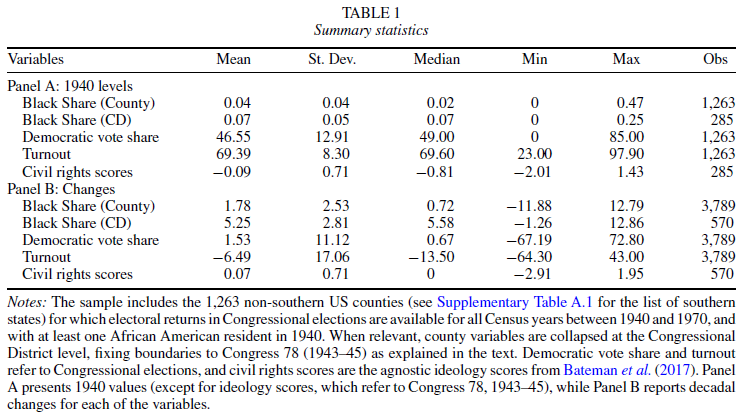
\includegraphics[scale = .5]{fig_tab/os20220708/T1.png}
  \end{figure}
\end{frame}

\begin{frame}{Descriptive Statistics}
  \begin{figure}
    \centering
    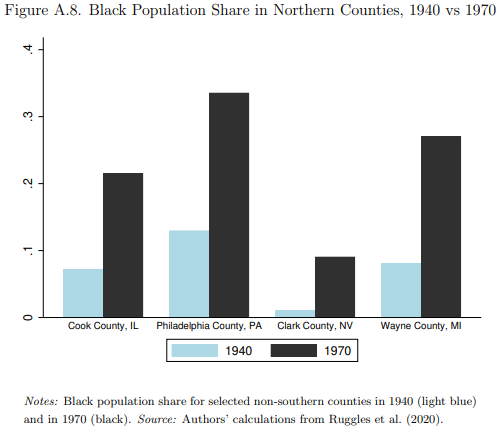
\includegraphics[scale = .5]{fig_tab/os20220708/FA8.png}
  \end{figure}
\end{frame}

\begin{frame}{Descriptive Statistics}
  \begin{figure}
    \centering
    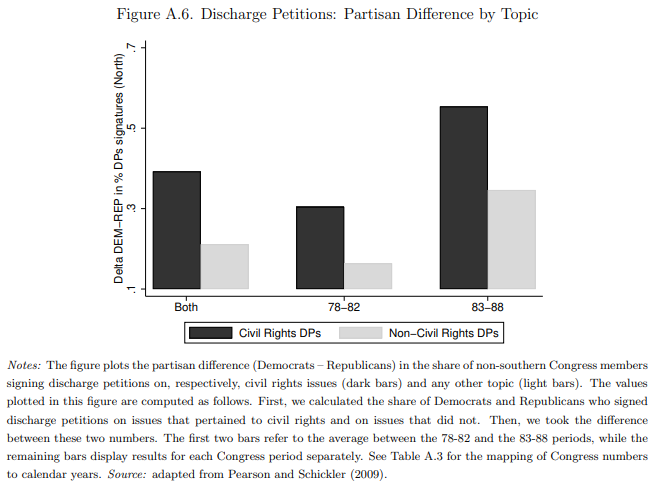
\includegraphics[scale = .45]{fig_tab/os20220708/FA6.png}
  \end{figure}
  \begin{itemize}
    \footnotesize
    \item While the poll tax and anti-discrimination employment (FECP) legislation were the most common topics during the 1940s, five of the eight discharge petitions filed between Congress 83 and Congress 88 concerned the CRA.
  \end{itemize}
\end{frame}

\section{Empirical Strategy}
\frame{\sectionpage}

\begin{frame}{Empirical Model}
  \begin{itemize}
    \item stacked first differences model for the three decades between 1940 and 1970:
    \begin{align*}
      \Delta y_{c \tau} = \delta_{s\tau} + \beta \Delta \text{BI}_{c \tau} + \gamma X_{c\tau} + u_{c \tau}
    \end{align*}
    \begin{itemize}
      \item for county $c$ in state $s$ during decade $\tau$.
      \item $\Delta y_{c \tau}$: change in the outcome of interest during the decade.
      \item $\Delta \text{BI}_{c \tau}$: the change in the Black population share
      \item $X_{c\tau}$: a vector of interactions between decade dummies and 1940 county characteristics.
      \item Weighted regression by 1940 county population do not change the main results.
      \item Standard errors are clustered at the county level.
    \end{itemize}
    \item In the CD-level analyses, they restrict attention to two periods: from Congress 78 (1943-45) to Congress 82 (1951-53); and, from Congress 82 (1951-53) to Congress 88 (1963-65).
  \end{itemize}
\end{frame}

\begin{frame}{Instrument for $\Delta \text{BI}_{c \tau}$}
  \begin{itemize}
    \item Black migrants might have sorted in places that were already undergoing economic and political changes
    
    $\Rightarrow$ the shift-share instrument (Card, 2001; Boustan, 2010)
    \begin{align*}
      Z_{c\tau} = \sum_{j \in \text{South}} sh_{jc} \text{BI}_{j\tau}
    \end{align*}
    \begin{itemize}
      \item for state $j$ during period $\tau$
      \item $sh_{jc}$ the share of Black migrants born in southern state $j$ and living in northern county $c$ in 1940
      \item $\text{BI}_{c \tau}$ number of Black migrants who left state $j$ during period $\tau$.
    \end{itemize}
    \item A large number of shocks are orthogonal to changes in outcomes in the destination (support for racial equality in non-southern counties) guarantee the validity of the shift-share design.
  \end{itemize}
\end{frame}

\section{Main Results}
\frame{\sectionpage}

\begin{frame}{Congressional Elections}
  \begin{figure}
    \centering
    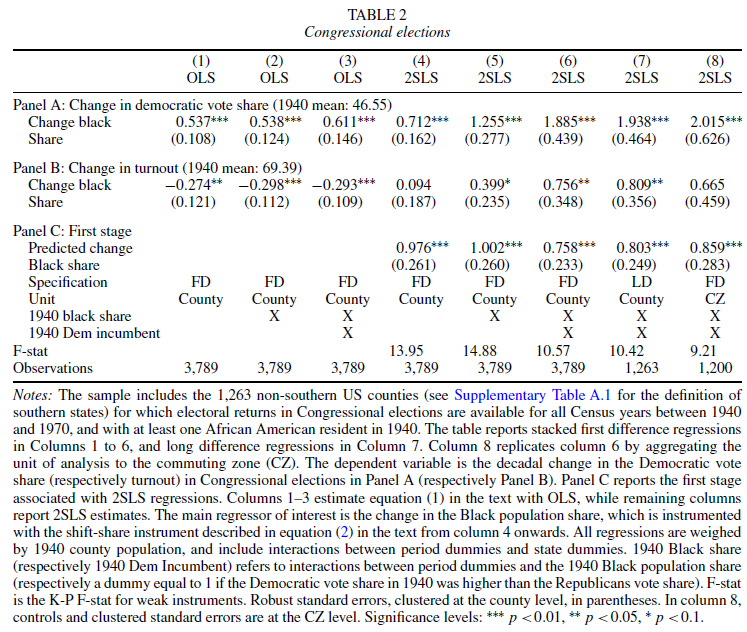
\includegraphics[scale = .4]{fig_tab/os20220708/T2.png}
  \end{figure}
\end{frame}

\begin{frame}{Congressional Elections}
  \begin{itemize}
    \item In all cases, the point estimate on the change in the Black population share is positive and statistically significant.
    \item 2SLS
    \begin{itemize}
      \item Instrument: Black population share raises the actual Black population share by 0.75 percentage points (Column 6).
      \item Effects are larger in magnitude.
    \end{itemize}
    \item one percentage point increase in the Black population share raised the Democratic vote share by 1.88 percentage points, or 4\% relative to the 1940 mean.
    \item Black migrants were quickly incorporated in the political life of northern and western counties.
  \end{itemize}
\end{frame}

\begin{frame}{Legislators' Ideology}
  \begin{figure}
    \centering
    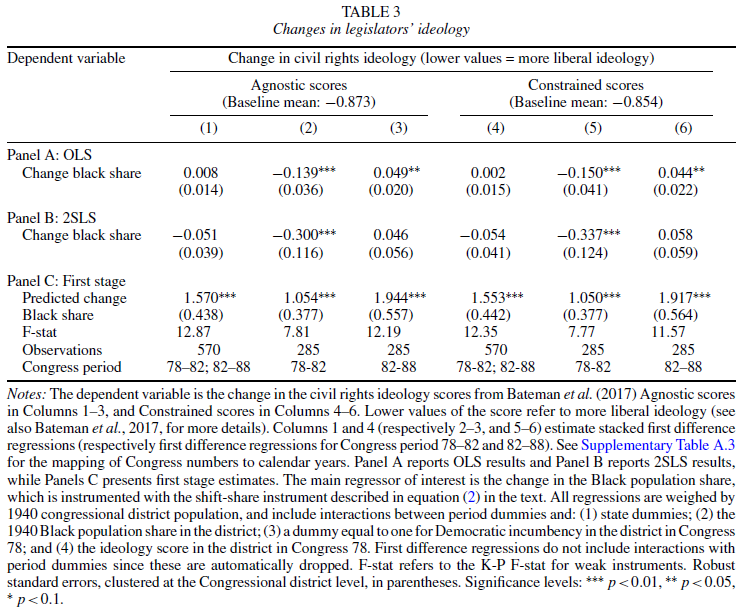
\includegraphics[scale = .4]{fig_tab/os20220708/T3.png}
  \end{figure}
\end{frame}

\begin{frame}{Signatures on Discharge Petitions}
  \begin{figure}
    \centering
    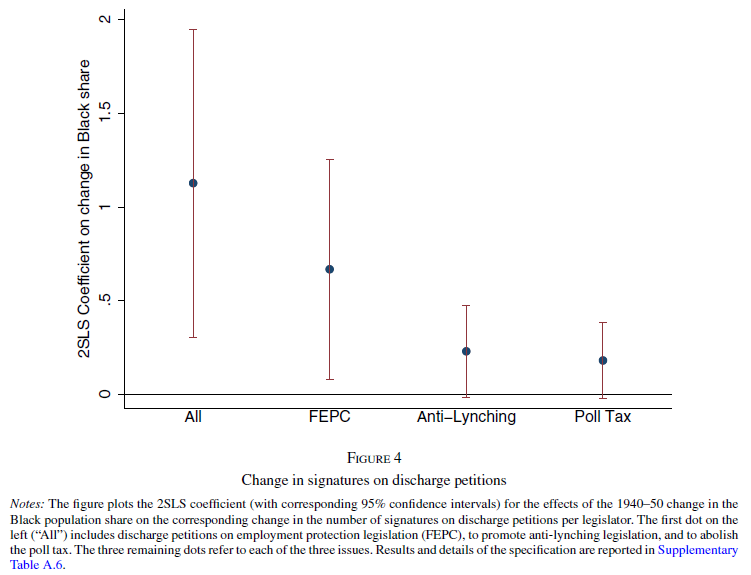
\includegraphics[scale = .5]{fig_tab/os20220708/F4.png}
  \end{figure}
\end{frame}

\begin{frame}{Legislators' Ideology}
  \begin{itemize}
    \item Ideology Scores:
    \begin{itemize}
      \item Black in-migration had a strong, negative effect on the ideology scores of legislators in the first Congress period (Column 2)
      \item On the other hand, a negligible, positive, and not statistically significant effect in the second period (Column 3).
    \end{itemize}
    \item Discharge Petitions:
    \begin{itemize}
      \item A first difference regression for the 78-82 Congress period
      \item Black in-migration increased the probability of signing a discharge petition on all topics: especially significant in FEPC (fair employment legislation)
      \item Black in-migration has no effect on the change in the probability of signing a discharge petition on non-civil rights topics
    \end{itemize}
  \end{itemize}
\end{frame}

\begin{frame}{Robustness Checks}
  \begin{itemize}
    \item Black in-migration did lead to white departures in central cities, but not in counties in their sample.
    \item lack inflows were not associated with changes in the composition of white residents and did not have any impact on whites' labour market outcomes
    \item County-to-county migration matrix to construct the initial shares does not change the results.
    \item The instrument is uncorrelated with two potential pull factors: WWII spending and New Deal relief programs.
    \item There are no pre-trends in the outcomes.
  \end{itemize}
\end{frame}

\section{Mechanisms}
\frame{\sectionpage}

\begin{frame}{Mechanisms}
  \begin{itemize}
    \item Black organizations and pro-civil rights activism
    \begin{itemize}
      \item Northern destinations of Black migrants also became centres of organized activism. (McAdam(1982) focused on the South).
    \end{itemize}
    \item White political preferences and racial atttidudes.
    \begin{itemize}
      \item The increase in the Democratic vote share documented in Section 5.1 cannot be explained by the inflow of Black migrants alone.
    \end{itemize}
  \end{itemize}
\end{frame}

\begin{frame}{Black Organizations and Pro-Civil Rights Activism}
  \begin{itemize}
    \item 2SLS results indicate that Black in-migration had no effect on the presence of the NAACP (the National Association for the Advancement of Colored People) as a whole
    \begin{itemize}
      \item However, effects turn to significant for counties that did not have a chapter in 1940 (Column 3).
      \item These identification do not capture the effects of Black in-migration on the change in the number of NAACP members.
    \end{itemize}
    \item The frequency of protests organized by CORE (Congress of Racial Equality) in support of civil rights are strongly affected by the Black migration.
    \begin{itemize}
      \item One percentage point increase in the Black population share leading to a 5.7 percentage point (more than 60\%) increase in the likelihood of protests
    \end{itemize}
  \end{itemize}
\end{frame}

\begin{frame}{NAACP Chapters and CORE Demonstrations}
  \begin{figure}
    \centering
    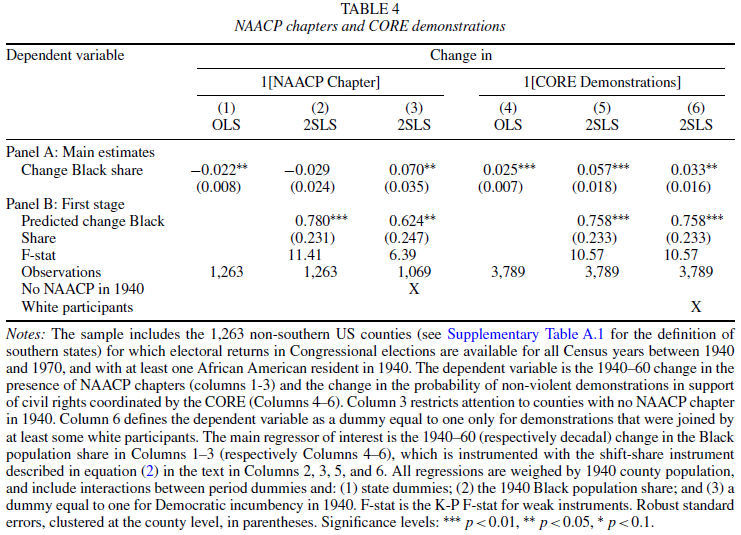
\includegraphics[scale = .5]{fig_tab/os20220708/T4.png}
  \end{figure}
\end{frame}

\begin{frame}{White Attitudes}
  \begin{itemize}
    \item Disaggregated data on voting behavior by race is not available.
    \item They rely instead on estimates of Black voting patterns from areas of selected cities whose residents were disproportionately Black (Chicago, Cincinnati, Cleveland, Detroit, Kansas City, New York City, Pittsburgh, and St. Louis). (Glantz, 1960)
    \begin{itemize}
      \item Using these cities, they estimated voting behaviour among Black residents in the Presidential elections of 1948, 1952, and 1956.
      \item Matching the estimated to each county, they calculate the number of white switchers per 10 Black inflows.
    \end{itemize}
    \item The implied number of white northern residents who would have to switch to the Democrats in 1960 in order to match the estimated effect of the increase in the Black population is 7 (per 10 Black migrants).
  \end{itemize}
\end{frame}

\begin{frame}{}
  \begin{figure}
    \centering
    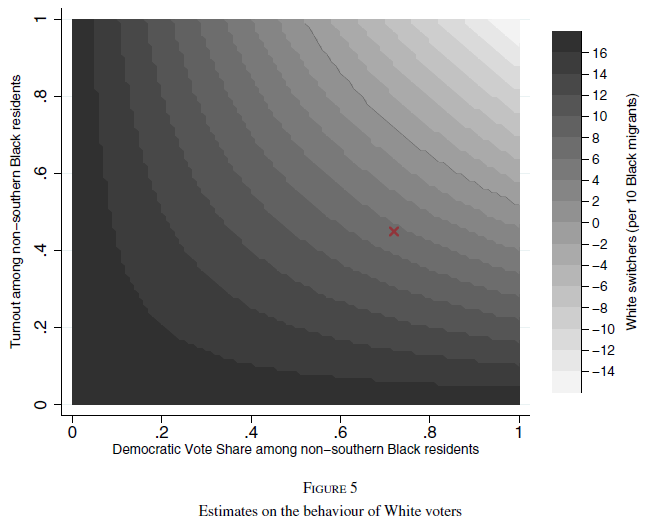
\includegraphics[scale = .5]{fig_tab/os20220708/F5.png}
  \end{figure}
\end{frame}

\begin{frame}{Evidence from Historical Data}
  \begin{itemize}
    \item American National Election Studies (ANES)
    \begin{itemize}
      \item individual-level responses and the respondent's race.
    \end{itemize}
    \item State-level analyses suggest a substansive effects between 1940 and 1960.
    \begin{itemize}
      \item one percentage point difference across states in the change in the Black population share implies a 3.3 percentage point (5\%relative to the mean) difference in respondents' thermometers.
    \end{itemize}
    \item Black in-migration also increases support for Civil rights and the Democratic party among white respondents (Column 5).
    \item White residents also participated in CORE demonstration (Column 6 in Table 4).
  \end{itemize}
\end{frame}

\begin{frame}{Whites' Attitude}
  \begin{figure}
    \centering
    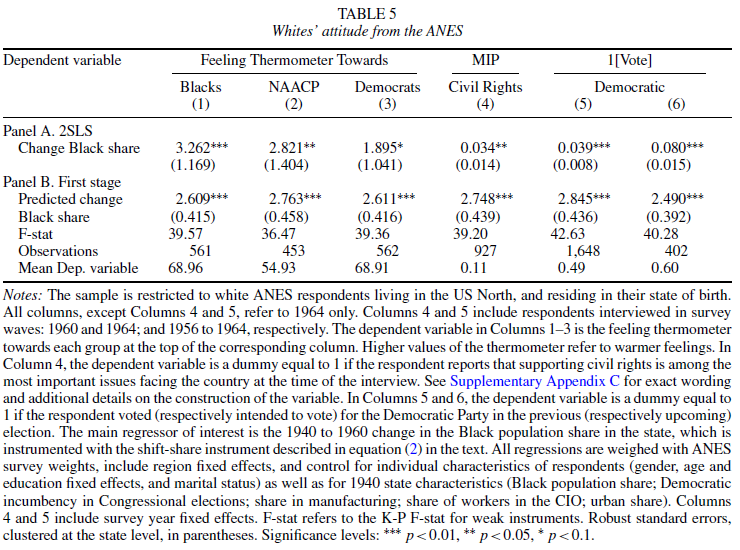
\includegraphics[scale = .5]{fig_tab/os20220708/T5.png}
  \end{figure}
\end{frame}

\begin{frame}{What Made the Whites Support Civil Rights?}
  \begin{itemize}
    \item Two prominent explanations identified by prior literature
    \begin{itemize}
      \item increased awareness of Black oppression in the South (Myrdal, 1944)
      \item the formation of a class-based cross-race coalition between white and Black members of the working class
    \end{itemize}
    \item Evidence on information transmission
    \begin{itemize}
      \item using a list of known lynchings against African Americans between 1940 and 1964 in the US South and non-southern newspapers.
    \end{itemize}
    \item Evidence on cross-race political coalition.
    \begin{itemize}
      \item Individual-level data from the ANES also support the idea of a cross-race coalition in which organized labour played a crucial role.
    \end{itemize}
  \end{itemize}
\end{frame}

\begin{frame}{Evidence on information transmission}
  \begin{itemize}
    \item Taking the dummy whether each lynching episode between 1940 and 1964 in the US South, is reported in 492 counties in 4-26 weeks.
    \begin{itemize}
      \item Thie dataset comprises a total of 1,041 newspapers, only five of which explicitly targeted an African American audience
    \end{itemize}
    \item Local newspapers of northern counties were more likely to report the episode in areas that had received more African Americans between 1940 and 1964.
    \item Event-study design revealed that the effect of Black in-migration jumps on the week of the lynching,
    and then gradually fades away, persisting for at least one month after the event.
  \end{itemize}
\end{frame}

\begin{frame}{}
  \begin{figure}
    \centering
    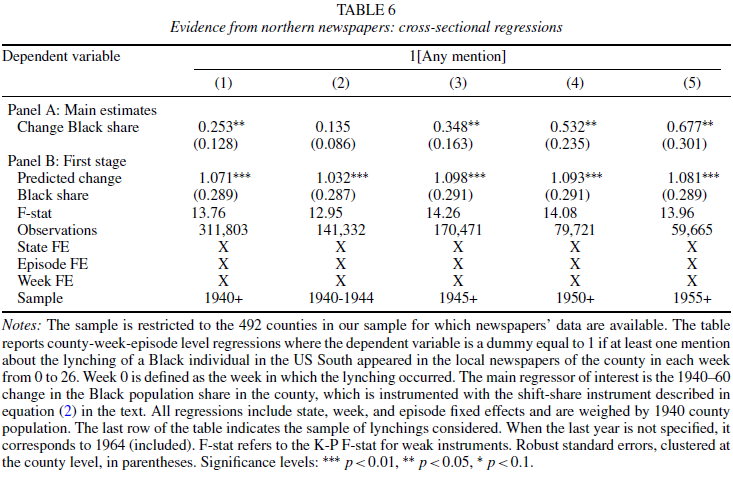
\includegraphics[scale = .5]{fig_tab/os20220708/T6.png}
  \end{figure}
\end{frame}

\begin{frame}{}
  \begin{figure}
    \centering
    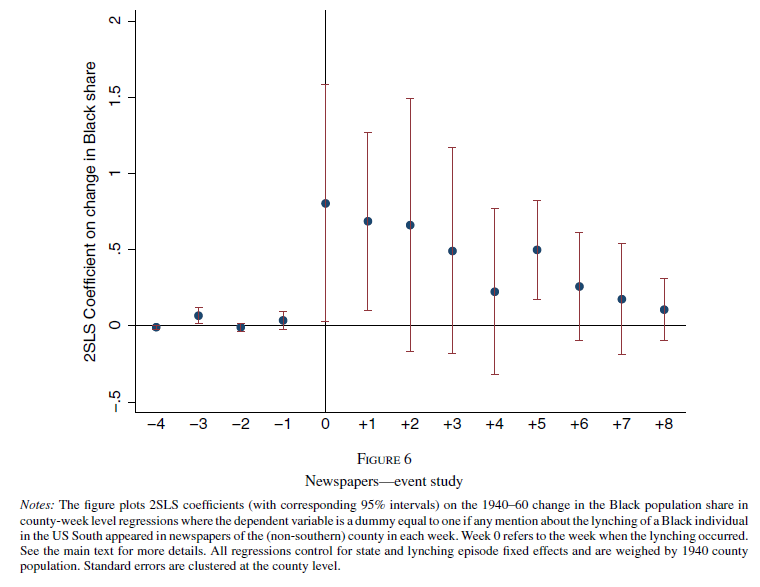
\includegraphics[scale = .5]{fig_tab/os20220708/F6.png}
  \end{figure}
\end{frame}

\begin{frame}{Crosspolitical coalition}
  \begin{itemize}
    \item Effect heterogeneity in county-specific characteristics.
    \begin{itemize}
      \item The surge in civil rights protests was in counties with a higher share of white workers in manufacturing.
      \item Pro-civil rights protests were also more frequent where political competition (measured by the margin of victory).
      \item Black in-migration led to more demonstrations only where predicted labour demand was stronger.
    \end{itemize}
    \item Findings are consistent with that the Great Migration had no effect on the Democratic vote share in the 1950s.
  \end{itemize}
\end{frame}

\begin{frame}{}
  \begin{figure}
    \centering
    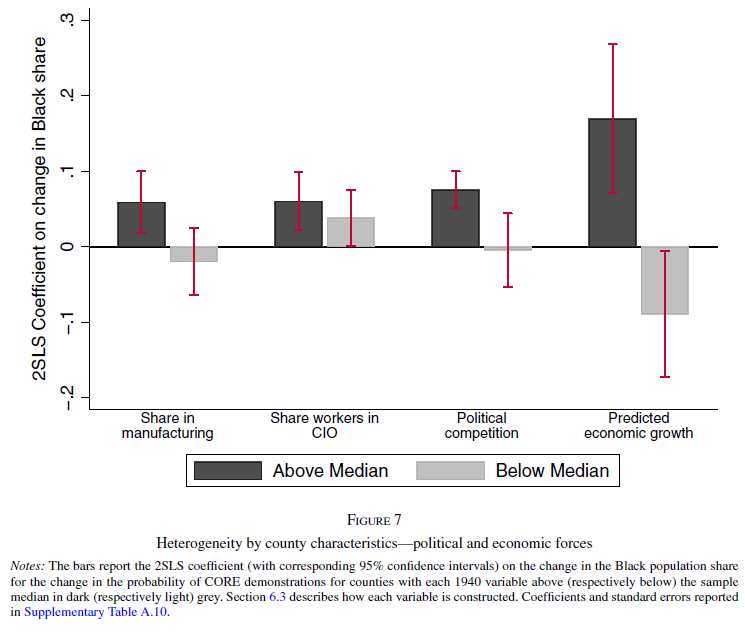
\includegraphics[scale = .5]{fig_tab/os20220708/F7.png}
  \end{figure}
\end{frame}

\begin{frame}{Additional Mechanisms}
  \begin{itemize}
    \item It is likely that similar dynamics were at play in radio and TV programs.
    \begin{itemize}
      \item It is possible that southern Black leaders strategically organized events in the South to attract attention of northern residents in migration destination counties.
    \end{itemize}
    \item Correlation between selective sorting of white residents and the patterns of Black migration: the spread of air conditioning during the 1960s made the South a more attractive destination for older white residents
    \item Effect heterogeneity
    \begin{itemize}
      \item An order of magnitude larger in counties with lower historical discrimination.
      \item Support for civil rights increased more in counties where inter-group contact in the housing market was lower.
    \end{itemize}
    \item Effects are persistent until today.
  \end{itemize}
\end{frame}

\section{Conclusions}
\frame{\sectionpage}

\begin{frame}{Conclusions}
  \begin{itemize}
    \item When contrasted with other works on the political effects of migration, our results raise an intriguing set of questions:
    \begin{itemize}
      \item Under what conditions can migration and inter-group contact more broadly lead to the formation of cross-group coalitions?
      
      : Cross-race cooperation can emerge when
      individuals belonging to different groups share similar goals and identities
      \item This likely facilitated support for racial equality among northern whites who were not materially affected.
    \end{itemize}
  \end{itemize}
\end{frame}

\end{document}
